\chapter{Results}
This section of the report shows the results of the tests performed on the chosen classifiers

\section{Preliminary Results}

The preliminary results were calculated on a subset of the MSTAR dataset; 1291 images spanning 5 classes were selected. Each image was cropped/padded to 100x100 pixels in size and then normalised, forming an input of 10,000 data points. No further processing was performed on the images.

The data was divided as follows: 85\% training, 5\% validation, 10\% testing. Instances are drawn randomly from the dataset without replacement. This is based on the idea that more training data results in a stronger classifier. The validation stage is for verifying the progress of the model and does not need too much data dedicated to it. Testing requires more data than validation - enough to confidently represent the contents of the entire dataset.

This resulted in a training set of 1097 images, a validation set of 64 images, and a test set of 129 images.

\subsection{Nearest Neighbour}
The Nearest Neighbour outperformed preliminary expectations, achieving 92.857\% classification accuracy on a test set of 322 instances. Each instance was compared to a dataset of 967 instances. The classification time for a single instance is 12.38 seconds.

\subsection{K-Nearest Neighbours}
Before optimising for K it was expected that a K value greater than K = 1 would provide the best results. After optimising, however, it was determined that K = 1 is indeed the optimal value for K, so the results were the same as the Nearest Neighbour classifier. Generating the squared distance matrix and calculating the optimal value of K constitutes the training time of KNN, which took 1.3 hours when testing for K up to 239 on a set of 967 100x100 images. The results of this optimisation are shown in Figure~\ref{fig:k_values}

\begin{figure}
	\centering
	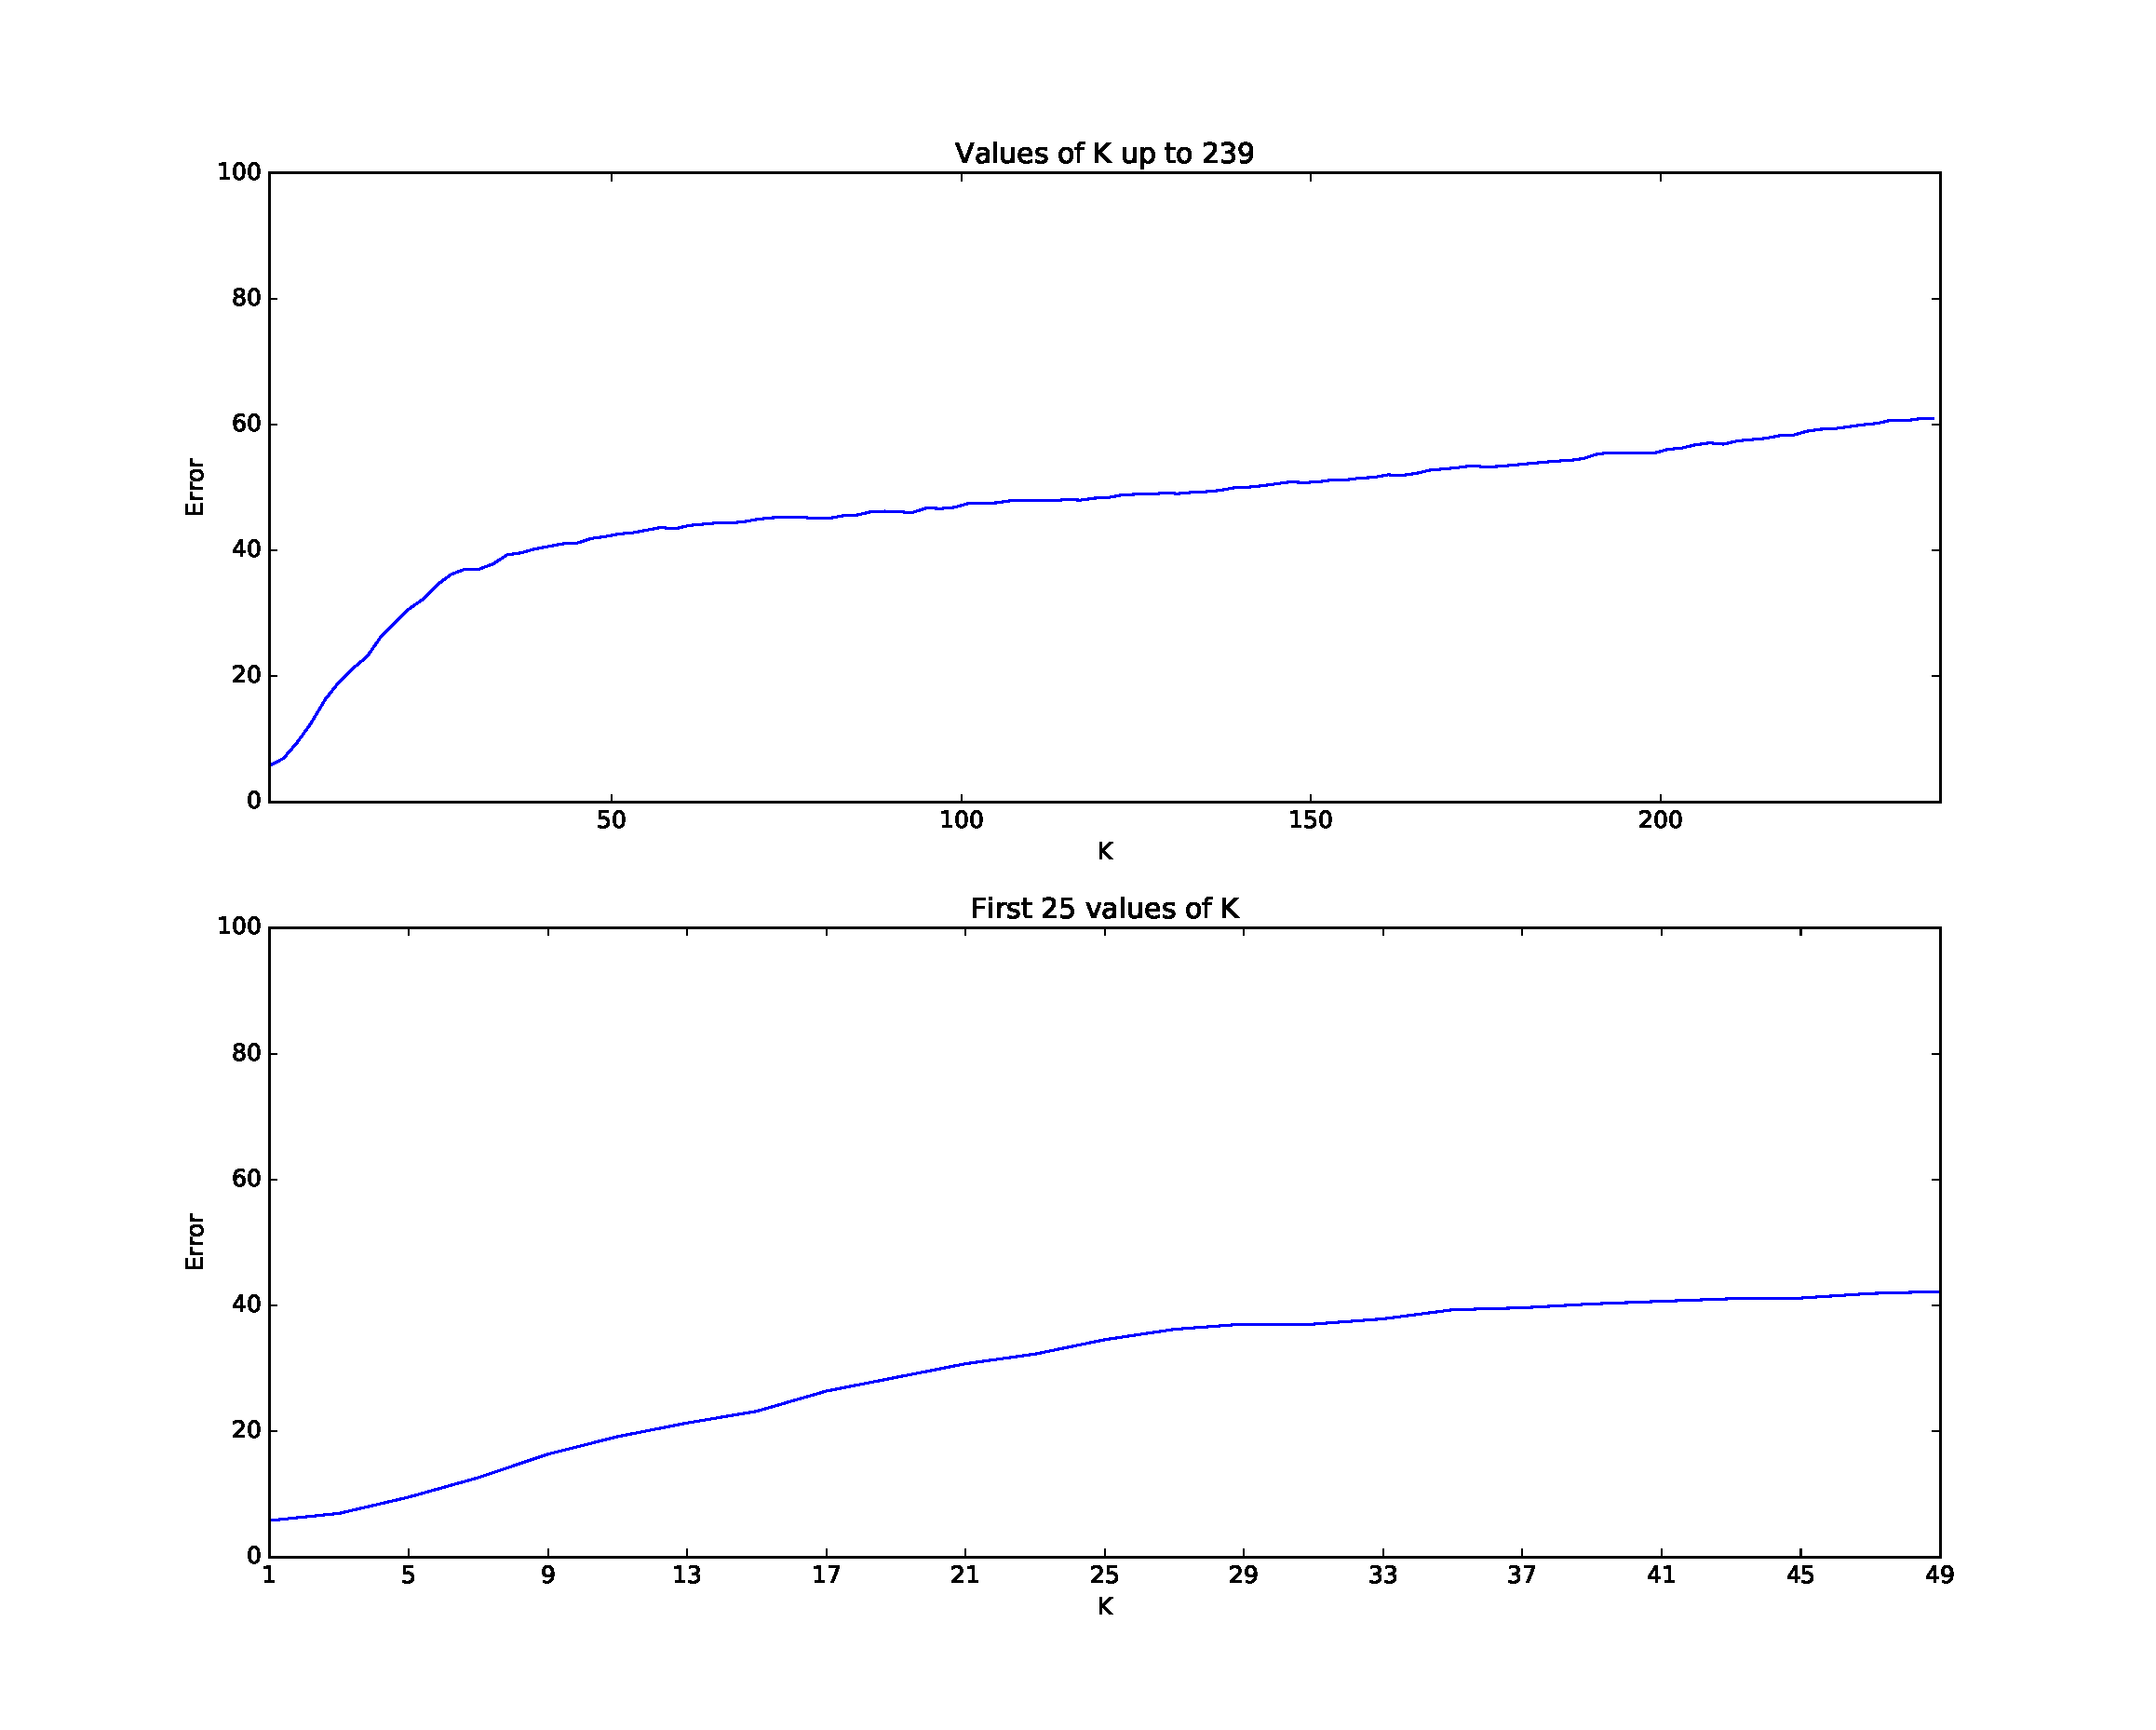
\includegraphics[width=\textwidth]{figures/k_values239}
	\caption{Optimising for K}
	\label{fig:k_values}
	\centering
\end{figure}

\subsection{Multilayer Perceptron}
The multilayer perceptron has the largest number of parameters that can be optimised, leading to a varied spread of results. The first parameters to optimise are the learning rate and the number of neurons in the hidden layer(s).

The learning rate controls how strongly the output error affects the shift in weight values every iteration. A smaller learning rate will typically cause the network to take longer to converge to its optimal weights, or get stuck in a local minimum, while a high learning rate can prevent the values from converging, resulting in oscillating values and no optimum being found.

The size of each hidden layer defines the number of connections between neurons. Too few connections can `bottleneck' the classifier, leaving it unable to extract any meaningful features. Too many connections can allow the classifier to extract more features, at the cost of a longer training time spent optimising the larger number of weights. It is predicted that too many connections can also lead to over-fitting of the classifier to the training dataset.

Preliminary results show that learning rate must be set in indirect proportion to the number of hidden neurons to maintain training and classification accuracy.

\subsubsection{Summary of Results}
The preliminary results obtained from testing on a reduced dataset are presented in Table~\ref{tab:prelim_results}. To assist with readability, important parameters are notated in brackets, for example MLP(10,5) denotes a Multilayer Perceptron with two hidden layers; 10 neurons in the first layer and 5 in the second. The training time for the KNN is optional, and should only be considered if an optimal K is found for the dataset.

The confusion matrix of the best-performing classifier is shown in Table~\ref{tab:prelim_conf}, demonstrating that the classification accuracy is already high after the preliminary results

\begin{table}
	\centering
	\begin{tabular}{|c|c|c|c|}
	
		\hline
		\textbf{Classifier} & \textbf{Training Time[s]} & \textbf{Classification Accuracy[\%]} & \textbf{Single-Instance Time} \\
		\hline
		KNN(k=1)		 & 0	  & 92.86 & 12.38s  \\ \hline
		KNN(k=3)		 & 0	  & 91.53 & 12.38s  \\ \hline
		KNN(k=1,trained) & 99.85  & 92.86 & 12.38s  \\ \hline
		MLP(10) 	     & 11.22  & 97.00 & 0.1ms   \\ \hline
		MLP(20) 	     & 42.97  & 96.33 & 0.074ms \\ \hline
		MLP(5,1)	     & 29.07  & 82.33 & 0.012ms \\ \hline
		MLP(5,5)	     & 7.58   & 98.33 & 0.087ms \\ \hline
		MLP(10,5)	     & 28.35  & 97.67 & 0.091ms \\ \hline
		MLP(10,10)       & 12.71  & 97.67 & 0.072ms \\ \hline
		MLP(5,5,5) 	     & 8.32   & 92.00 & 0.064ms \\ \hline
		MLP(10,10,10)    & 20.77  & 91.67 & 0.068ms \\ \hline
	
	\end{tabular}
	\caption{Preliminary Results}
	\label{tab:prelim_results}
	\centering
\end{table}

\section{Preliminary Comments}
Analysis of the preliminary results gives direction to the development of each classifier. It can immediately be seen that the KNN classifier is outclassed by even a roughly optimised Multilayer Perceptron. 

\subsection{K-Nearest Neighbours}\label{sec:knn_results}
The K-Nearest Neighbour classifier results are intended to function only as a low benchmark and point of reference, so its design remains unchanged. Comparing it to the Multilayer Perceptron shows that a Nearest Neighbour approach is infeasible for large datasets and large instances of data. No further testing needs to be performed to establish this.

\subsection{Multilayer Perceptron}

The required hidden layer size is much smaller than anticipated; a single hidden layer with 5 neurons performs adequately. Optimisation of the weights according to their L2 norm proved crucial in improving predictive accuracy while reducing the cost of the classifier. A crude grid search was used to find the best L2 regularisation parameter, which was chosen as 0.1. The training time of each MLP is not directly proportional to the number of neurons. Single-class classification time for all MLP models is suitable for real-time application. Some of the classifiers have met and exceeded the design specifications in Section~\ref{sec:design_spec}.

\subsection{Data}
The division of the dataset between training, validation and testing should remain at 85\% training, 5\% validation, 10\% testing. Preliminary results have given no evidence that suggests a change in the allocation of data.


\section{Final Results}

\subsection{Data Processing}
The input images are rescaled to match at least the size of the largest images in dataset (192x193), and so are resized to 194x194. Thresholding is used to reduce the clutter present in each radar image. The threshold chosen is the median of each image. The full dataset is used, totalling 4459 images, 8 classes, with the training:validation:testing ratio at 85:5:10. This results in a training set of 3790 images, a validation set of 222 images, and a test set of 445 images.


\subsection{K-Nearest Neighbours}
As stated in Section~\ref{sec:knn_results}, no further testing of the KNN classifier needs to be done to prove that it is inferior to the Multilayer Perceptron. However, to provide additional context, it was decided that the single-instance classification time should be measured on the full dataset. It takes 193.82 seconds to run a single instance against every instance in the training dataset. Definitely infeasible.


\subsection{Multilayer Perceptron}
The MLP performs exceedingly well on a larger dataset  and with larger input images. Classification accuracy of 100\% is achieved, meeting and exceeding the design specifications in Section~\ref{sec:design_spec}.



\subsection{Summary of Results}

The final results of the report are shown in Table~\ref{tab:final_results}. To assist with readability, important parameters are notated in brackets, for example MLP(10,5) denotes a Multilayer Perceptron with two hidden layers; 10 neurons in the first layer and 5 in the second. The confusion matrix corresponding to the best classifier is shown in Table~\ref{tab:final_conf}.

\section{Final Comments}
\subsection{K-Nearest Neighbours}
As stated in Section~\ref{sec:knn_results}, the KNN classifier is not suitable for the task at hand. It scales too poorly with the size of the dataset, and does not provide a classification high enough to justify the long classification times that are introduced.

\subsection{Multilayer Perceptron}

The required hidden layer size is much smaller than anticipated; a single hidden layer with 5 neurons is enough to achieve 100\% classification. The introduction of more neurons and hidden layers does not lead to improved accuracy, although one or two hidden layers of 5 to 10 neurons each appears to be the `sweet spot'. Introducing too many layers or neurons can prevent the weights from converging to local minima during training, leading to the low classification accuracy in MLP(5,5,5) and  MLP(10,10,10). They remained entirely untrained.

\subsection{Data}
The division of the dataset between training, validation and testing should remain at 85\% training, 5\% validation, 10\% testing. Preliminary results have given no evidence that suggests a change in the allocation of data.

\subsection{Classifier Robustness}
The best-performing classifier was trained again on data with additive Gaussian noise. The classification accuracy was reduced from 100\% to 99.52\%. This is within the design specifications in Section~\ref{sec:design_spec}.

\subsection{Future Improvements}
Moving forward, implementing more complex neural networks that can deal with non-centred images is critical. Convolutional neural networks are outside the scope of this report, but deal well with off-centre images.

\begin{table}
	\centering
	\begin{tabular}{|c|c|c|}
		\hline
		\textbf{Class} & \textbf{No. Images} & \textbf{Suffix} \\
		\hline
		2S1        & 573 & 000 \\ \hline
		BRDM       & 572 & 001 \\ \hline
		BTR 60     & 451 & 003 \\ \hline
		D7         & 573 & 005 \\ \hline
		SLICY      & 572 & 015 \\ \hline
		T62        & 572 & 016 \\ \hline
		ZIL131     & 573 & 025 \\ \hline
		ZSU\_23\_4 & 573 & 026 \\ \hline	
	\end{tabular}
	\caption{Input Data}
	\label{tab:input_data}
	\centering
\end{table}

\begin{table}
	\centering
	\begin{tabular}{|c|c|c|c|}
		
		\hline
		\textbf{Classifier} & \textbf{Training Time[s]} & \textbf{Classification Accuracy[\%]} & \textbf{Single-Instance Time} \\
		\hline
		KNN(k=1)		 & -----	   & -----  & 193.82s \\ \hline
		MLP(5) 	     	 & 16.47   & 100.00 & 0.174ms   \\ \hline
		MLP(10) 	     & 23.24   & 100.00 & 0.156ms   \\ \hline
		MLP(20) 	     & 45.22   & 96.33  & 0.156ms \\ \hline
		MLP(5,1)	     & 749.58  & 92.14  & 0.978ms \\ \hline
		MLP(10,5)	     & 66.19   & 99.76  & 0.185ms \\ \hline
		MLP(10,10)       & 66.64   & 99.76  & 0.206ms \\ \hline
		MLP(5,2,1) 	     & 745.72  & 92.14  & 0.175ms \\ \hline
		MLP(5,5,5) 	     & 7.93    & 11.00  & 0.127ms \\ \hline
		MLP(10,10,10)    & 11.60   & 11.00  & 0.226ms \\ \hline
		
	\end{tabular}
	\caption{Preliminary Results}
	\label{tab:final_results}
	\centering
\end{table}


\begin{table}
	\centering
	\begin{tabular}{|*{11}{c|}}
		
		\cline{3-10}
		\multicolumn{2}{c|}{}         & \multicolumn{8}{|c|}{Predicted Class} 			\\ \cline{3-10}
		\multicolumn{2}{c|}{}                  & 2S1 & BRDM & BTR 60 & D7 & SLICY & T62 & ZIL131 & ZSU\_23\_4 \\ \hline
		\multirow{8}{*}{\begin{turn}{90}Actual Class\end{turn}}
				        & 2S1        & 99.56 & 0.44 & 0 & 0 & 0 & 0 & 0 & 0 	\\ \cline{2-10}
                        & BRDM       & 0 & 100 & 0 & 0 & 0 & 0 & 0 & 0 	\\ \cline{2-10}
                        & BTR 60     & 0 & 0 & 100 & 0 & 0 & 0 & 0 & 0 	\\ \cline{2-10}
                        & D7 	     & 0 & 0 & 0 & 100 & 0 & 0 & 0 & 0 	\\ \cline{2-10}
                        & SLICY      & 0 & 0 & 0 & 0 & 100 & 0 & 0 & 0 	\\ \cline{2-10}
                        & T62        & 0 & 0 & 0 & 0 & 0 & 100 & 0 & 0 	\\ \cline{2-10}
                        & ZIL131 	 & 0 & 0 & 0 & 0 & 0 & 0 & 100 & 0 	\\ \cline{2-10}
                        & ZSU\_23\_4 & 0 & 0 & 0 & 0 & 0 & 0 & 0 & 100 	\\ \cline{2-10} 
		\hline	\end{tabular}
	\label{tab:prelim_conf}
	\caption{Preliminary Confusion Matrix}
	\centering
\end{table}

\begin{table}
	\centering
	\begin{tabular}{|*{11}{c|}}
		
		\cline{3-10}
		\multicolumn{2}{c|}{}         & \multicolumn{8}{|c|}{Predicted Class} 			\\ \cline{3-10}
		\multicolumn{2}{c|}{}                  & 2S1 & BRDM & BTR 60 & D7 & SLICY & T62 & ZIL131 & ZSU\_23\_4 \\ \hline
		\multirow{8}{*}{\begin{turn}{90}Actual Class\end{turn}}
		& 2S1        & 100 & 0 & 0 & 0 & 0 & 0 & 0 & 0 	\\ \cline{2-10}
		& BRDM       & 0 & 100 & 0 & 0 & 0 & 0 & 0 & 0 	\\ \cline{2-10}
		& BTR 60     & 0 & 0 & 100 & 0 & 0 & 0 & 0 & 0 	\\ \cline{2-10}
		& D7 	     & 0 & 0 & 0 & 100 & 0 & 0 & 0 & 0 	\\ \cline{2-10}
		& SLICY      & 0 & 0 & 0 & 0 & 100 & 0 & 0 & 0 	\\ \cline{2-10}
		& T62        & 0 & 0 & 0 & 0 & 0 & 100 & 0 & 0 	\\ \cline{2-10}
		& ZIL131 	 & 0 & 0 & 0 & 0 & 0 & 0 & 100 & 0 	\\ \cline{2-10}
		& ZSU\_23\_4 & 0 & 0 & 0 & 0 & 0 & 0 & 0 & 100 	\\ \cline{2-10} 
		\hline	\end{tabular}
	\label{tab:final_conf}
	\caption{Final Confusion Matrix}
	\centering
\end{table}

